\chapter{Signal selection}
\label{ch:ana-sig}

\par In this analysis, in order to obtain a high signal over background efficiencies, the physics object-level selection is applied first, then, signal regions are designed. 
Moreover, control regions are defined to constrain the background contribution.

\section{Physics object definition}
\label{sec:ana-sig:physobj}

\subsection{Leptons}

\begin{itemize}
    \item \textbf{Electrons}: As described in Section~\ref{sec:el}, electrons can be identified using various likelihood-based criteria, for example, shower profile selections, track quality, and high threshold TRT hits. The electron identification criteria that are used in this analysis are listed In Table~\ref{tab:c7:physobj:ele}.
    \item \textbf{Muons}: Muons are reconstructed with combined information from the inner tracker and muon spectrometer. Moreover, two different working points are applied in this analysis for muon identification. A loose criterion is applied as baseline muon selection to obtain larger acceptance, while the medium working point is used in signal selection for higher purity. More details are listed in Table~\ref{tab:c7:physobj:muo}.
    \item \textbf{$\tau$-Leptons}: As described in Section~\ref{sec:taus}, $\tau$-lepton is reconstructed using the inner tracker and calorimeter. Since events with $\tau$-leptons are vetoed in both signal and control regions, a loose $\tau$-lepton working point is enough for this analysis. More information can be found in Table~\ref{tab:c7:physobj:tau}.
\end{itemize}

\begin{table}[ht]
    \caption{Electron selection criteria.}
    \label{tab:c7:physobj:ele}
    \centering
    \begin{tabular}{|c|c|}
        \hline
        Feature & Criterion \\
        \hline
        \hline
        Pseudorapidity range & \(|\eta| < 2.47\) \\
        \hline
        Transverse momentum & \pt~$>$~7~\GeV~\\
        \hline
        Track to vertex association & \(|d_{0}^{\text{BL}}(\sigma)| < 5\)\\ & \(|\Delta z_{0}^{\text{BL}} \sin{\theta}| < 0.5mm\) \\
        \hline
        Identification & \texttt{FCLoose} \\
        \hline
        Isolation & \texttt{LooseTrackOnly / FCHighPtCaloOnly} \\
        \hline
    \end{tabular}
\end{table}

\begin{table}[ht]
    \caption{Muon selection criteria.}
    \label{tab:c7:physobj:muo}
    \centering
    \begin{tabular}[ht]{|c|c|c|}
        \hline
        Feature & Baseline criterion & Signal criterion \\
        \hline
        \hline
        Selection working point & \texttt{Loose} & \texttt{Medium} \\
        \hline
        Isolation working point & \texttt{FCLoose} &  \texttt{FCTightTrackOnly} \\
        \hline
        Momentum calibration & Sagitta correction & Sagitta correction \\
        \hline
        \pt~cut & 7~\GeV~& 7~\GeV~\\ 
        \(|\eta|\) cut & \(< 2.7\) & \(< 2.5\) \\
        \hline
        \(d_{0}\) significance cut & 3 & 3 \\
        \hline
        \(z_{0}\) cut & 0.5mm & 0.5mm \\
        \hline
    \end{tabular}
\end{table}

\begin{table}[ht]
    \caption{Tau selection criteria.}
    \label{tab:c7:physobj:tau}
    \centering
    \begin{tabular}{|c|c|}
        \hline
        Feature & Criterion \\
        \hline
        \hline
        Pseudorapidity range & \(|\eta| < 2.5\) \\
        \hline
        Track selection & 1 or 3 tracks \\
        \hline
        Charge & \(|Q| = 1\) \\
        \hline
        Tau energy scale & \texttt{MVA TES} \\
        \hline
        Transverse momentum & \pt~$>$~20~\GeV~\\
        \hline
        Jet rejection & BDT-based (\texttt{Loose}) \\
        \hline
        Electron rejection & BDT-based \\
        \hline
        Muon rejection & \specialcell{Via overlap removal in \(\Delta R < 0.2\) and \pt~$>$~>2~\GeV.\\ Muons must not be Calo-tagged} \\
        \hline
    \end{tabular}
\end{table}

\subsection{Jets}

\begin{itemize}
    \item \textbf{Small-radius jets}: As mentioned in Section~\ref{sec:jets}, small-radius jets can be divided into two categories: central jets and forward jets. In this analysis, only the central jets are used to reconstruct the Higgs boson, while both central and forward jets are involved in the \met~calculation. More details about small-radius jet identification can be found in Table~\ref{tab:c7:physobj:srjets}.
    \item \textbf{Large-radius jets}: The large-radius jets are reconstructed with large cone size (R=1.0). These large cone size jets are used to reconstruct the boosted Higgs boson. More details are listed in Table~\ref{tab:c7:physobj:lrjets}.
    \item \textbf{Variable-radius track jets}: The variable-radius track jets are reconstructed from the inner tracker data using the anti-$k_{t}$ algorithm. The jet radius is dependent on the jet \pt: $R=\frac{30~\GeV}{p_{T}}$. The variable-radius track jets provide a better acceptance when reconstructing boosted Higgs bosons in this analysis.
    \item \textbf{b-jets}: $b$-tagging is a technology to identify the b-jets, which is applied on central jets to reconstruct the resolved Higgs boson. More detailed information can be found in Table~\ref{tab:c7:physobj:bjets}.
\end{itemize}

\begin{table}[ht]
    \caption{Small-\(R\) jet reconstruction criteria.}
    \label{tab:c7:physobj:srjets}
    \centering
    \begin{tabular}{|c|c|}
        \hline
        Feature & Criterion \\
        \hline
        \hline
        Algorithm & Anti-$k_{t}$ \\
        \hline
        \(R\)-parameter & 0.4 \\
        \hline
        Input constituent & PFlow \\
        \hline
        \texttt{CalibArea} tag & 00-04-82 \\
        \hline
        Calibration configuration & \specialcell{\texttt{JES\_MC16Recommendation\_}\\\texttt{Consolidated\_EMTopo\_Apr2019\_Rel21.config}} \\
        \hline
        Calibration sequence (Data) & \texttt{JetArea\_Residual\_EtaJES\_GSC\_Insitu} \\
        \hline
        Calibration sequence (MC) & \texttt{JetArea\_Residual\_EtaJES\_GSC} \\
        \hline
        Jet cleaning & \texttt{TightBad} \\
        \hline
        \pt~& \(> 20~\GeV\) (central) / \(> 30~\GeV\) (forward) \\
        \hline
        \(|\eta|\) & \(< 2.5\) (central) /  \(2.5 < |\eta| < 4.5 \) (forward) \\
        \hline
        JVT & \specialcell{\texttt{Medium} working point,\\applied only to central jets with \pt~$<$~120~\GeV} \\
        \hline
    \end{tabular}
\end{table}
    
\begin{table}[ht]
    \caption{Large-\(R\) jet reconstruction criteria.}
    \label{tab:c7:physobj:lrjets}
    \centering
    \begin{tabular}{|c|c|}
        \hline
        Feature & Criterion \\
        \hline
        \hline
        Algorithm & Anti-$k_{t}$ \\
        \hline
        R-parameter & 1.0 \\
        \hline
        Input constituent & \texttt{LCTopo} \\
        \hline
        Grooming algorithm & Trimming \\
        \hline
        Subjet \pt~fraction for trimming & 0.05 \\
        \hline
        \(R_{\text{trim}}\) & 0.2 \\
        \hline
        \texttt{CalibArea} tag & 00-04-82 \\
        \hline
        Calibration configuration (Data) & \specialcell{\texttt{JES\_MC16recommendation\_FatJet}\\\texttt{\_Trimmed\_JMS\_comb\_3April2019.config}} \\
        \hline
        Calibration configuration (MC) & \specialcell{\texttt{JES\_MC16recommendation\_FatJet}\_\\\texttt{Trimmed\_JMS\_comb\_17Oct2018.config}} \\
        \hline
        Calibration sequence (Data) & \texttt{EtaJES\_JMS\_Insitu} \\
        \hline
        Calibration sequence (MC) & \texttt{EtaJES\_JMS} \\
        \hline
        \pt~& \(> 200~\GeV\) \\
        \hline
        \(|\eta|\) & \(< 2\) \\
        \hline
    \end{tabular}
\end{table}

\begin{table}[ht]
    \caption{b-jets selection criteria.}
    \label{tab:c7:physobj:bjets}
    \centering
    \begin{tabular}{|c|c|}
        \hline
        Feature & Criterion \\
        \hline
        \hline
        Jet collection & \texttt{AntiKt4EMPFlow / AntiKtVR30Rmax4Rmin02} \\
        \hline
        Algorithm & \texttt{DL1} \\
        \hline
        Operating point & Eff = 77 \\
        \hline
        CDI & \texttt{2017-21-13TeV-MC16-CDI-2019-07-30\_v1} \\
        \hline
    \end{tabular}
\end{table}
  
\subsection{Missing transverse momentum}

\par As described in Section~\ref{sec:met}, the missing transverse momentum (\met) is defined as the magnitude of the missing transverse momentum vector, which is calculated using all well-reconstructed physics object, like the electron, muon, and jets. 
More information about the \met~selection for this analysis is listed in Table~\ref{tab:c7:physobj:met}.

\begin{table}[ht]
    \caption{\met~reconstruction criteria.}
    \label{tab:c7:physobj:met}
    \centering
    \begin{tabular}{|c|c|}
        \hline
        Parameter & Value \\
        \hline
        \hline
        Algorithm & Calo-based \\
        \hline
        Soft term & Track-based (TST) \\
        \hline
        \met~operating point & \texttt{Tight} \\
        \hline
    \end{tabular}
\end{table}

\section{Signal regions}
\label{sec:ana-sig:sigreg}
\par Signal regions are a set of phase spaces defined by a combination of selection conditions for signal selection. 
In this analysis, the most important signature is the Higgs boson, which has different signatures at different energy scales. 
Therefore, resolved and merged regions are designed as sub-signal regions to probe signals effectively at different Higgs boson momenta.

\subsection{Common event selection}
\par Several common event selection criteria are applied for both resolved and merged regions as a baseline selection.
\begin{itemize}
    \item \textbf{Event cleaning}: Event cleaning applies a set of filters to veto corrupted or noisy events. In this analysis, LAr noise burst, tile corruption, SCT recovery procedure, and incomplete events are applied as the event cleaning filters. More information can be found in Ref~\cite{c8-evt-cleaning}.
    \item \textbf{Loose jet Veto}: In the analysis, reconstructed jets can due to noise, collision background, etc.. The TightBadJet criterion, provided by the Jet/\met~group, is applied in this analysis to veto events that contain fake jets.
    \item \textbf{\met~selection}: In signal regions, a constraint \met~~$>$~150~\GeV~is applied. In control regions, the lepton momentum is treated as part of the missing transverse momentum and the same \met~cut is applied.
    \item \textbf{Light lepton and $\tau$-lepton veto}: Events that contain a electron, muon or $\tau$-lepton, as defined in Section~\ref{sec:ana-sig:physobj}, are rejected.
    \item \textbf{Extended $\tau$-lepton veto}: An extended $\tau$ veto is applied in case a $\tau$-lepton failed to be identified. A hadronically decayed $\tau$ can be viewed as a jet. Therefore, a jet is considered as a $\tau$ candidate if it fulfills two conditions: (1) The track multiplicity in the jet cone is between 1 and 4. (2) The azimuthal separation between the jet and \met~is $\Delta \phi \leq 22.5^\circ$. The cut on the track multiplicity in the jet cone makes sure that the hadronic decay products in the jet are compatible with $\tau$-lepton decay products, namely with charged pions. The tracks considered are required to be associated with the primary vertex and have \pt~greater than 1 ~\GeV. The cut on the angular separation between the jet and \met~selects $\tau$-candidates that come from W bosons.
    \item \textbf{$\min_{j \in \{1,2,3\}}\Delta\phi(E_{\mathrm{T}}^{\mathrm{miss}},j)$ selection}: QCD multijet events can pass the \met~requirement because of incorrect jet energy measurement. In the case of fake \met, the \met~will generally point in the direction of leading jets. Therefore, an angular cut between \met~and leading jets is applied to veto these events.
\end{itemize}

\par After this baseline selection, the signal regions need to be analyzed different sub-regions based on the Higgs boson signature. 
In the target model, the sum of the \met~vector and Higgs boson transverse momentum vector should be zero-based on momentum conservation. 
Therefore, one can apply a single cut on \met~to separate events with resolved or merged Higgs bosons. In this analysis, the cut \met~$<$~500~\GeV~selects the resolved region while \met~$>$~500~\GeV~defines the merged region. Higgs boson identification, which will be detailed in the rest of this section, is different in these two signal regions.
\par Moreover, there is one additional condition to select events with at least one b-jet. $b$-tagging is applied on all small-radius central jets in the resolved region, but only on the two leading track jets that are associated with large-radius jets in the merged region.

\subsection{Resolved region}

\par In the resolved region, the Higgs boson momentum is relatively low. Therefore, the Higgs boson decay products, two $b$-jets, can be resolved into two separate jets. To reconstruct the Higgs boson, a set of jet candidates needs to be selected first. There are two categories in the Higgs boson jet candidate set: (1) $b$-tagged jets, (2) central non-$b$-tagged jets. The jets are ordered in decreasing transverse momentum within each category. The first two from each set of jets (referred to as j1 and j2 below) are used to reconstruct the Higgs boson candidate, which is referred to as $H_{reco}$.

\par There are several criteria to select the Higgs boson in the resolved channel:

\begin{itemize}
    \item \textbf{\pt~of $H_{reco}$}: This is expected to increase with \met. Therefore, a selection \pt$(H_{reco})>$~100~\GeV~is applied when \met~$<$~350~\GeV, while \pt$(H_{reco}) >$~300~\GeV~is required when 350~\GeV~$<$~\met~$<$~500~\GeV.
    \item \textbf{$m_{jj}$}: A window around the mass of the reconstructed Higgs boson is helpful to identify the Higgs boson. The mass of the reconstructed Higgs boson can be calculated from the invariant mass of the jet pair ($m_{jj}$) that forms $H_{reco}$. A window 50~\GeV~$< m_{jj} <$~280~\GeV~is applied in this analysis. 
    \item \textbf{$m_{T}^{b}$}: In the resolved region, the major background is top quark pair production. $m_{T}^{b}$ is introduced to reject these background events. $m_{T}^{b}$ is defined as: $m_{T}^{b}=\sqrt{2p_{T}^{b}E_{T}^{miss}(1-cos\Delta\phi(\vec{p}_{T}, \vec{E}_{T}^{miss}))}$. $m_{T}^{b}$ is calculated using the $b$-jets that are closest to and furthest from \met. The closest $b$-jet $m_{T}^b$ is required to be greater than 170~\GeV, while the furthest must be greater than 200~\GeV.
\end{itemize}

\par In addition, it is possible that the measured \met~of an event is due to a resolution fluctuation. Therefore, a \met~significance cut $S > 12$ is introduced to reject fake \met~events.

\subsection{Merged region}

\par In the merged region, the momentum of the Higgs boson is relatively high, and therefore, the decay products are close to each other in the lab frame and can be merged into a single cone, which is reconstructed as a large-radius jet in the detector.
\par Several criteria are applied on the large-radius jet to identify the Higgs boson in the merged region:
\begin{itemize}
    \item \textbf{$m_{J}$}: The invariant mass of the large-radius jet is an expression of Higgs boson mass. A window 50~\GeV~$< m_{J} <$ ~270~\GeV~is applied.
    \item \textbf{Variable-radius track jets association}: At least two variable-radius track jets need to be associated with the large-radius jet.
\end{itemize}

\par As a summary of Section~\ref{sec:ana-sig:sigreg}, both resolved and merged signal region selections are listed in Table~\ref{tab:c7:sigreg:summary}.

\begin{table}[h]
    \centering
    \begin{center}
        \begin{tabular}{cc}
            \hline
            \textbf{Resolved} & \textbf{Merged} \\
            \hline
            \hline
            \multicolumn{2}{c}{lowest unprescaled \met~trigger} \\
            \hline
            \multicolumn{2}{c}{veto on baseline light leptons and $\tau$-leptons} \\
            \hline
            \multicolumn{2}{c}{extended $\tau$-veto} \\
            \hline
            \multicolumn{2}{c}{\met~$>$ 150~\GeV} \\
            \hline
            \multicolumn{2}{c}{$\mindphi > 20^\circ$} \\
            \hline
            \met~$<$~500~\GeV~& \met~$>$~500~\GeV~\\
            \hline
            N(central small-R jets) $\geq$ 2 & N(central large-R jets) $\geq$ 1 \\
            \hline
            N($b$-tagged small-R jets) $\geq 1$ & N($b$-tagged associated track jets) $\geq 1$ \\
            \hline
            S $>$ 12 & --- \\
            \hline
            \pt$(jj) >$ 100~\GeV~if \met~$<$~350~\GeV~& --- \\
            \hline
            \pt$(jj) >$ 300~\GeV~if \met~$\geq$ 350~\GeV~& --- \\
            \hline
            $\mtb{\min} >$ 170~\GeV& --- \\
            \hline
            $\mtb{\max} >$ 200~\GeV& --- \\
            \hline
            50~\GeV~$< m_{jj} <$~280~\GeV~& 50~\GeV~$< m_{J} <$~270~\GeV~\\
            \hline
            $b$-tagging on small-radius jets & $b$-tagging on variable-radius track jets \\
            \hline
        \end{tabular}
    \end{center}
    \caption{Summary of the resolved and merged event selections applied in the 0-lepton channel. $\mathcal{S}$ denotes the object based \met~significance.}
    \label{tab:c7:sigreg:summary}
\end{table}

\section{Control regions}
\label{sec:ana-sig:ctlreg}
\par Control regions are a set of phase spaces that are orthogonal to the signal regions. 
Control regions are designed to validate the background estimate in the signal regions.

\subsection{1-lepton control region}
\par In the signal region, the W + jets background is mostly composed of events in which the $W$-boson decays leptonically. 
The $t\bar{t}$ background in the signal region originates almost completely from semileptonic $t\bar{t}$ decays. 
Events with leptons can enter the signal region if the leptons fail to be identified or if they are outside the detector acceptance. 
The largest contribution comes from decays involving $\tau$-leptons, as shown in Figure~\ref{fig:ttbarDecayCat}. 
Figure~\ref{fig:ttbarDecayCatKinematic} shows the distributions of different kinematic variables for the dominant decay modes. 
From there, it can be seen that shapes of the event variables agree well within the statistical uncertainties. 
Therefore the W+jets and $t\bar{t}$ backgrounds can be estimated using a 1-lepton control region, in which the lepton could have any flavor in principle.

\begin{figure}[h]
    \centering
    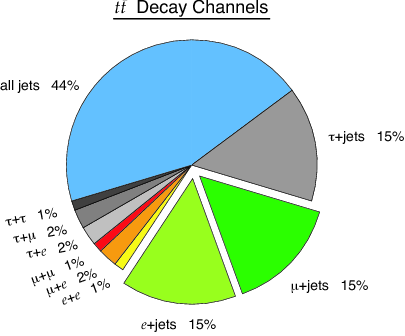
\includegraphics[width=0.9\textwidth]{chapters/c7/figures/ttbar-decay-modes.png}
    \caption{Decay categories for $t\bar{t}$ events. The classification of the decay processes was performed by examining the truth particle information within the reconstructed signal region events. The three dominant decay modes are the semileptonic decays with either a light lepton, a leptonically or a hadronically decaying $\tau$-lepton.}
    \label{fig:ttbarDecayCat}
\end{figure}

\begin{figure}[h]
    \centering
    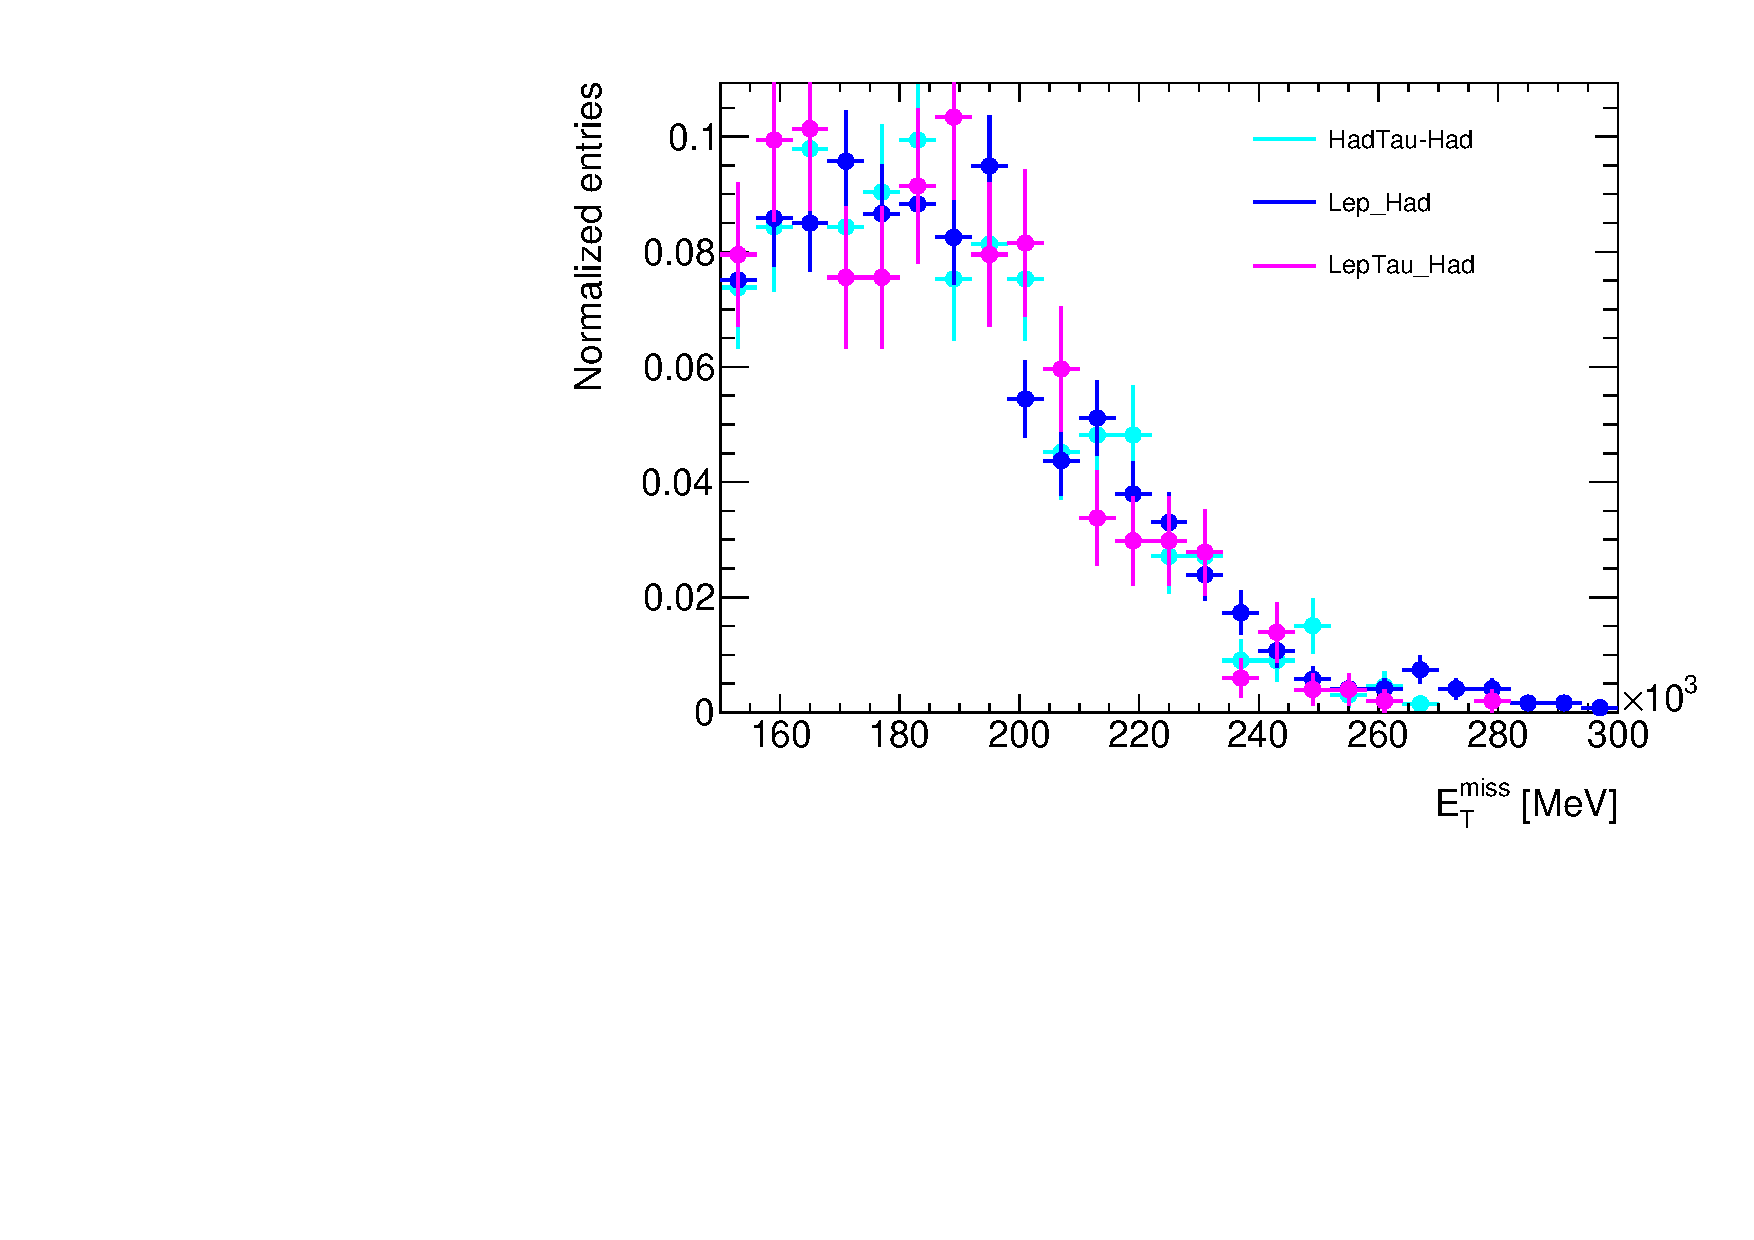
\includegraphics[width=0.45\textwidth]{chapters/c7/figures/ttbar_MetTST_met.pdf}
    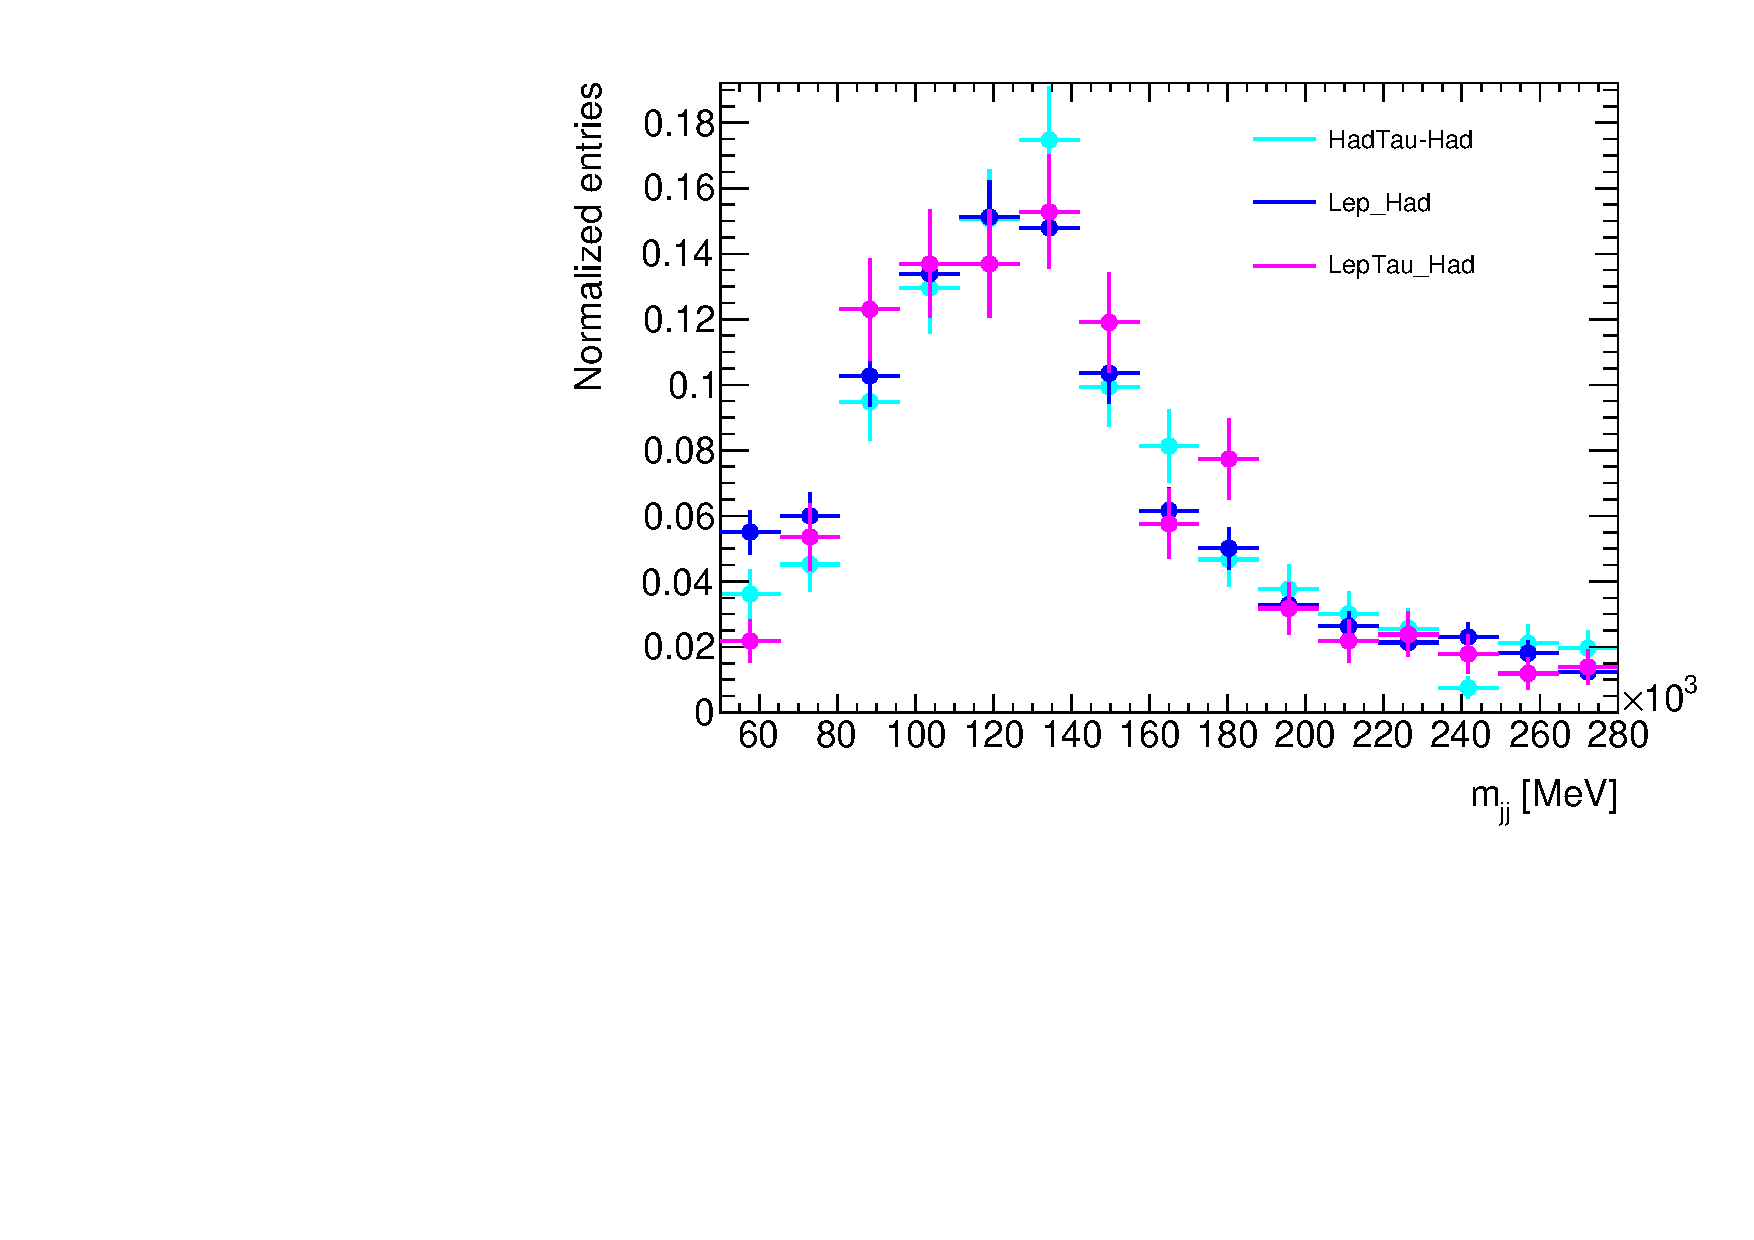
\includegraphics[width=0.45\textwidth]{chapters/c7/figures/ttbar_m_jj.pdf}
    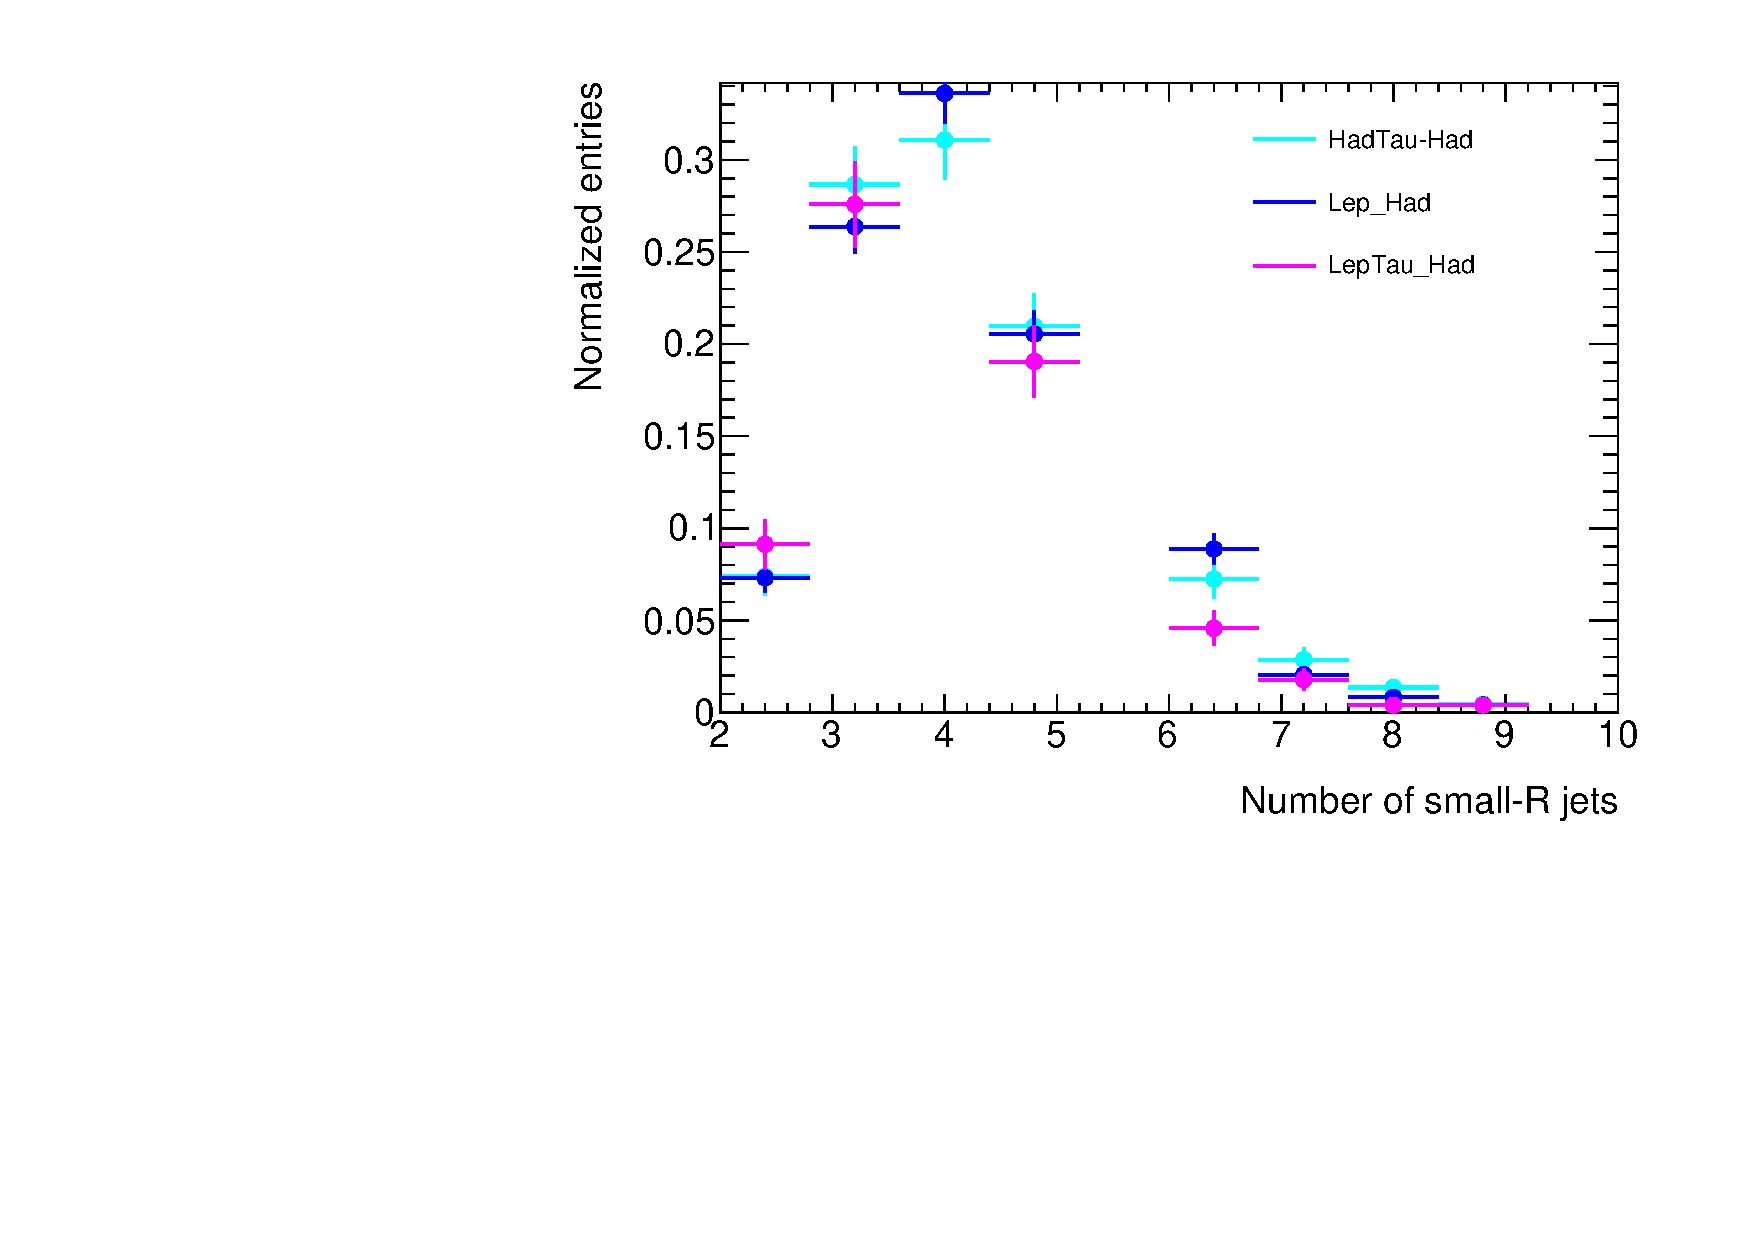
\includegraphics[width=0.45\textwidth]{chapters/c7/figures/ttbar_N_Jets04.pdf}      
    \caption{Normalised distributions of \met, the Higgs boson candidate mass and the number of small-radius jets for $t\bar{t}$ events. The distributions are shown separately for the three semileptonic decay modes, which are the dominant decays modes in the signal region.}
    \label{fig:ttbarDecayCatKinematic}
\end{figure}

\par The 1-muon control region is chosen to constrain W + jets related background. Events in this control region are required to have exactly one muon and no other baseline leptons.

\subsection{2-lepton control region}
\par A 2-lepton control region is used to estimate the Z +jets background. 
In the signal region the $Z(\to\nu\nu)+jets$ production leads to a significant amount of background, which has the topology as $Z(\to\ell\ell)+jets$ because the momentum of the $Z$ boson does not depend on its decay products. 
Hence the normalisation of $Z(\to\nu\nu)+jets$ events can be estimated with the help of a $Z(\to\ell\ell)+jets$ control region.

\par The 2-lepton control region is defined by selecting exactly two muons or two electrons. 
At least one of the leptons needs to satisfy the signal lepton criteria with sufficiently high \pt~to pass the trigger. 
The leading muon is required to have \pt~$>$~25~\GeV, while the leading electron is \pt~$>$~27~\GeV. 
The other lepton is not required to pass the signal lepton selection to increase acceptance. 
Moreover, since the two leptons originate from a $Z$ boson, a mass window requirement is implemented to identify the $Z$ mass peak: $|m_{Z}-m_{ll}|<$~10~\GeV.
